% This is an included file. See the master file for more information.
%
% When editing this file:
%
%    1. To change formatting, appearance, or style, please edit openmp.sty.
%
%    2. Custom commands and macros are defined in openmp.sty.
%
%    3. Be kind to other editors -- keep a consistent style by copying-and-pasting to
%       create new content.
%
%    4. We use semantic markup, e.g. (see openmp.sty for a full list):
%         \code{}     % for bold monospace keywords, code, operators, etc.
%         \plc{}      % for italic placeholder names, grammar, etc.
%
%    5. There are environments that provide special formatting, e.g. language bars.
%       Please use them whereever appropriate.  Examples are:
%
%         \begin{fortranspecific}
%         This is text that appears enclosed in blue language bars for Fortran.
%         \end{fortranspecific}
%
%         \begin{note}
%         This is a note.  The "Note -- " header appears automatically.
%         \end{note}
%
%    6. Other recommendations:
%         Use the convenience macros defined in openmp.sty for the minor headers
%         such as Comments, Syntax, etc.
%
%         To keep items together on the same page, prefer the use of 
%         \begin{samepage}.... Avoid \parbox for text blocks as it interrupts line numbering.
%         When possible, avoid \filbreak, \pagebreak, \newpage, \clearpage unless that's
%         what you mean. Use \needspace{} cautiously for troublesome paragraphs.
%
%         Avoid absolute lengths and measures in this file; use relative units when possible.
%         Vertical space can be relative to \baselineskip or ex units. Horizontal space
%         can be relative to \linewidth or em units.
%
%         Prefer \emph{} to italicize terminology, e.g.:
%             This is a \emph{definition}, not a placeholder.
%             This is a \plc{var-name}.
%


\section{Canonical Loop Form}
\label{sec:Canonical Loop Form}
\index{canonical loop form}
\begin{ccppspecific}
A loop has \emph{canonical loop form} if it conforms to the following:

\medskip
\nolinenumbers
\renewcommand{\arraystretch}{1.0}
\tablefirsthead{%
    \hline\\[-2ex]
    \multicolumn{2}{l}{\hspace*{-5pt}%
        \code{for (\plc{init-expr}; \plc{test-expr}; \plc{incr-expr}) \plc{structured-block}}}\\[2pt]
    \hline\\[-2ex]
}
\tablehead{%
    \multicolumn{2}{l}{\small\slshape continued from previous page}\\
    \hline\\[-2ex]
}
\tabletail{%
    \hline\\[-2ex]
    \multicolumn{2}{l}{\small\slshape continued on next page}\\
}
\tablelasttail{\hline}
\begin{supertabular}{ p{0.8in} p{4.5in}}
    \plc{init-expr} & One of the following:\\
    & \plc{var} = \plc{lb}\\
    & \plc{integer-type} \plc{var} = \plc{lb}\\
    & \plc{random-access-iterator-type} \plc{var} = \plc{lb}\\
    & \plc{pointer-type} \plc{var} = \plc{lb}\\
    & \\
    \plc{test-expr} & One of the following:\\
    & \plc{var} \plc{relational-op} \plc{b}\\
    & \plc{b} \plc{relational-op} \plc{var}\\
    & \\
    \plc{incr-expr} & One of the following:\\
    & ++\plc{var}\\
    & \plc{var}++\\
    & {-} {-} \plc{var}\\
    & \plc{var {-} {-}}\\
    & \plc{var} += \plc{incr}\\
    & \plc{var} {-} = \plc{incr}\\
    & \plc{var} = \plc{var} + \plc{incr}\\
    & \plc{var} = \plc{incr} + \plc{var}\\
    & \plc{var} = \plc{var} - \plc{incr}\\
    & \\
    \plc{var} & One of the following:\\
    & \hspace{1.5em}A variable of a signed or unsigned integer type.\\
    & \hspace{1.5em}For C++, a variable of a random access iterator type.\\
    & \hspace{1.5em}For C, a variable of a pointer type.\\
    & If this variable would otherwise be shared, it is implicitly made private in the loop 
    construct. This variable must not be modified during the execution of the \plc{for-loop} 
    other than in \plc{incr-expr}. Unless the variable is specified \code{lastprivate}
    or \code{linear} on the loop construct, its value after the loop is unspecified.\\
    \plc{relational-op} & One of the following:\\
    & \code{<}\\
    & \code{<=}\\
    & \code{>}\\
    & \code{>=}\\
    & \code{!=}\\
    & \\
    \plc{lb} and \plc{b} & Loop invariant expressions of a type compatible with the type of \plc{var}.\\
    & \\
    \plc{incr} & A loop invariant integer expression.\\
\end{supertabular}
\linenumbers
\medskip

% blue line floater at top of this page for "Fortran, cont."
\begin{figure}[t!]
    \linewitharrows{-1}{dashed}{C/C++ (cont.)}{8em}
\end{figure}
The canonical form allows the iteration count of all associated loops to be computed 
before executing the outermost loop. The computation is performed for each loop in an 
integer type. This type is derived from the type of \plc{var} as follows:

\begin{itemize}
    \item If \plc{var} is of an integer type, then the type is the type of \plc{var}.
    
    \item For C++, if \plc{var} is of a random access iterator type, then the type is the type that 
    would be used by \plc{std::distance} applied to variables of the type of \plc{var}.
    
    \item For C, if \plc{var} is of a pointer type, then the type is \code{ptrdiff\_t}.
\end{itemize}

The behavior is unspecified if any intermediate result required to compute the iteration 
count cannot be represented in the type determined above.

There is no implied synchronization during the evaluation of the \plc{lb}, \plc{b}, or \plc{incr} 
expressions. It is unspecified whether, in what order, or how many times any side effects 
within the \plc{lb}, \plc{b}, or \plc{incr} expressions occur.

\begin{note}
Random access iterators are required to support random access to elements in 
constant time. Other iterators are precluded by the restrictions since they can take linear 
time or offer limited functionality. It is therefore advisable to use tasks to parallelize 
those cases. 

% The word "Restrictions" seems out of place; was it meant to be a header outside of the Note?

%Restrictions
\end{note}

\restrictions
The following restrictions also apply:

\begin{itemize}
    \item If \plc{test-expr} is of the form \plc{var} \plc{relational-op} 
    \plc{b} and \plc{relational-op} is < or <= then \plc{incr-expr} must cause \plc{var} to increase on each 
    iteration of the loop. If \plc{test-expr} is of 
    the form \plc{var} \plc{relational-op} \plc{b} and \plc{relational-op} 
    is > or >= then \plc{incr-expr} must cause \plc{var} to decrease on each iteration of the loop.
    
    \item If \plc{test-expr} is of the form \plc{b} \plc{relational-op} 
    \plc{var} and \plc{relational-op} is < or <= then 
    \plc{incr-expr} must cause \plc{var} to decrease on each iteration of the loop. If \plc{test-expr} is of 
    the form \plc{b} \plc{relational-op} \plc{var} and \plc{relational-op} 
    is > or >= then \plc{incr-expr} must cause \plc{var} to increase on each iteration of the loop.
    
    \item For C++, in the \code{simd} construct the only random access iterator types that are 
    allowed for \plc{var} are pointer types.
    
    \item The \plc{b}, \plc{lb} and \plc{incr} expressions may not reference
    \plc{var} of any of the associated loops.

    \item If \plc{relational-op} is != and \plc{incr-expr} is of the
    form that has \plc{incr} then \plc{incr} must be equal to 1.
\end{itemize}
\end{ccppspecific}





\section{Worksharing Constructs}
\label{sec:Worksharing Constructs}
\index{worksharing constructs}
\index{constructs!worksharing}
\index{worksharing!constructs}
A worksharing construct distributes the execution of the associated region among the 
members of the team that encounters it. Threads execute portions of the region in the 
context of the implicit tasks each one is executing. If the team consists of only one 
thread then the worksharing region is not executed in parallel.

A worksharing region has no barrier on entry; however, an implied barrier exists at the 
end of the worksharing region, unless a \code{nowait} clause is specified. If a \code{nowait} 
clause is present, an implementation may omit the barrier at the end of the worksharing 
region. In this case, threads that finish early may proceed straight to the instructions 
following the worksharing region without waiting for the other members of the team to 
finish the worksharing region, and without performing a flush operation. 

The OpenMP API defines the following worksharing constructs, and these are described 
in the sections that follow:

\begin{itemize}
\item loop construct

\item \code{sections} construct

\item \code{single} construct

\item \code{workshare} construct
\end{itemize}

\begin{samepage}
\restrictions
The following restrictions apply to worksharing constructs:

\begin{itemize}
\item Each worksharing region must be encountered by all threads in a team or by none at 
all, unless cancellation has been requested for the innermost enclosing parallel 
region.

\item The sequence of worksharing regions and \code{barrier} regions encountered must be the 
same for every thread in a team
\end{itemize}
\end{samepage}










\subsection{Loop Construct}
\label{subsec:Loop Construct}
\index{loop@{\code{loop}}}
\index{constructs!loop@{\emph{loop}}}
\index{constructs!do@{\code{do} \emph{Fortran}}}
\index{do@{\code{do}, \emph{Fortran}}}
\index{for@{\code{for}, \emph{C/C++}}}
\index{constructs!for@{\code{for}, \emph{C/C++}}}
\summary
The loop construct specifies that the iterations of one or more associated loops will be 
executed in parallel by threads in the team in the context of their implicit tasks. The 
iterations are distributed across threads that already exist in the team executing the 
\code{parallel} region to which the loop region binds.

\syntax
\begin{ccppspecific}
The syntax of the loop construct is as follows:

\begin{boxedcode}
\#pragma omp for \plc{[clause[ [},\plc{] clause] ... ] new-line} 
    \plc{for-loops}
\end{boxedcode}

where clause is one of the following: 
\index{clauses!collapse@{\code{collapse}}}

\begin{indentedcodelist}
private(\plc{list})
firstprivate(\plc{list})
lastprivate(\plc{[ lastprivate-modifier}:\plc{] list})
linear(\plc{list[ }:\plc{ linear-step]})
reduction(\plc{reduction-identifier }:\plc{ list})
schedule(\plc{[modifier [}, \plc{modifier]}:\plc{]kind[},\plc{ chunk\_size]})
collapse(\plc{n})
ordered\plc{[}(\plc{n})\plc{]}
nowait
\end{indentedcodelist}

The \code{for} directive places restrictions on the structure of all associated \plc{for-loops}. 
Specifically, all associated \plc{for-loops} must have \emph{canonical loop form} (see 
\specref{sec:Canonical Loop Form}).
\end{ccppspecific}

\begin{fortranspecific}
The syntax of the loop construct is as follows:

\begin{boxedcode}
!\$omp do \plc{[clause[ [},\plc{] clause] ... ]}
   \plc{do-loops}
\textsl{[}!\$omp end do \textsl{[}nowait\textsl{]]}
\end{boxedcode}

where \plc{clause} is one of the following:

\begin{indentedcodelist}
private(\plc{list})
firstprivate(\plc{list})
lastprivate(\plc{[ lastprivate-modifier}:\plc{] list})
linear(\plc{list[ }:\plc{ linear-step]})
reduction(\plc{reduction-identifier }:\plc{ list})
schedule(\plc{[modifier [}, \plc{modifier]}:\plc{]kind[},\plc{ chunk\_size]})
collapse(\plc{n})
ordered\plc{[}(\plc{n})\plc{]}
\end{indentedcodelist}

If an \code{end}~\code{do} directive is not specified, an \code{end}~\code{do} directive is assumed at the end of the 
\plc{do-loops}.

Any associated \plc{do-loop} must be a \plc{do-construct} or an
\plc{inner-shared-do-construct} as defined by the Fortran standard. If
an \code{end}~\code{do} directive follows a \plc{do-construct} in
which several loop statements share a \code{DO} termination statement,
then the directive can only be specified for the outermost of these
\code{DO} statements.

If any of the loop iteration variables would otherwise be shared, they are implicitly 
made private on the loop construct.
\end{fortranspecific}


\binding
The binding thread set for a loop region is the current team. A loop region binds to the 
innermost enclosing \code{parallel} region. Only the threads of the team executing the 
binding \code{parallel} region participate in the execution of the loop iterations and the 
implied barrier of the loop region if the barrier is not eliminated by a \code{nowait} clause.

\descr
The loop construct is associated with a loop nest consisting of one or more loops that 
follow the directive.

There is an implicit barrier at the end of a loop construct unless a \code{nowait} clause is 
specified.

\index{clauses!collapse@{\code{collapse}}}
The \code{collapse} clause may be used to specify how many loops are 
associated with the loop construct. The parameter of the \code{collapse} 
clause must be a constant positive integer expression. If a \code{collapse} 
clause is specified with a parameter value greater than 1, then the 
iterations of the associated loops to which the clause applies are collapsed 
into one larger iteration space that is then divided according 
to the \code{schedule} clause. The sequential execution of the iterations 
in these associated loops determines the order of the iterations in the 
collapsed iteration space. If no \code{collapse} clause is present or its 
parameter is 1, the only loop that is associated with the loop construct 
for the purposes of determining how the iteration space is divided according 
to the \code{schedule} clause is the one that immediately follows the 
loop directive. 

The iteration count for each associated loop is computed before entry to the 
outermost loop. If execution of any associated loop changes any of the values 
used to compute any of the iteration counts, then the behavior is unspecified.

The integer type (or kind, for Fortran) used to compute the iteration count 
for the collapsed loop is implementation defined.

\index{clauses!schedule@{\code{schedule}}}
A worksharing loop has logical iterations numbered 0,1,...,N-1 where N is the 
number of loop iterations, and the logical numbering denotes the sequence in 
which the iterations would be executed if a set of associated loop(s) were 
executed sequentially. The \code{schedule} clause specifies how iterations of 
these associated loops are divided into contiguous non-empty subsets, called 
chunks, and how these chunks are distributed among threads of the team. Each 
thread executes its assigned chunk(s) in the context of its implicit task. 
The iterations of a given chunk are executed in sequential order by the assigned thread.
The \plc{chunk\_size} expression is evaluated using the original list items of 
any variables that are made private in the loop construct. It is unspecified 
whether, in what order, or how many times, any side effects of the evaluation 
of this expression occur. The use of a variable in a \code{schedule} clause 
expression of a loop construct causes an implicit reference to the variable 
in all enclosing constructs.

Different loop regions with the same schedule and iteration count, even if 
they occur in the same parallel region, can distribute iterations among 
threads differently. The only exception is for the \code{static} schedule 
as specified in Table~\ref{tab:Schedule-Values}. Programs that depend 
on which thread executes a particular iteration under any other circumstances 
are non-conforming. 

See \specref{subsubsec:Determining the Schedule of a Worksharing Loop} 
for details of how the schedule for a worksharing loop is 
determined. 

The schedule \plc{kind} can be one of those specified in 
Table~\ref{tab:Schedule-Values}.

The schedule \plc{modifier} can be one of those specified in 
Table~\ref{tab:Schedule Clause Modifier Values}. If the 
\code{static} schedule kind is specified or if the \code{ordered} 
clause is specified, and if the \code{nonmonotonic} modifier is 
not specified, the effect is as if the \code{monotonic} modifier 
is specified. Otherwise, unless the \code{monotonic} modifier is 
specified, the effect is as if the \code{nonmonotonic} modifier 
is specified.

The \code{ordered} clause with the parameter may also be used to specify 
how many loops are associated with the loop construct. The parameter of 
the \code{ordered} clause must be a constant positive integer expression
if specified. The parameter of the \code{ordered} clause does not
affect how the logical iteration space is then divided. If an \code{ordered} 
clause with the parameter is specified for the loop construct, then those 
associated loops form a \emph{doacross loop nest}. 

If the value of the parameter in the \code{collapse} or \code{ordered} 
clause is larger than the number of nested loops following the construct, 
the behavior is unspecified.

\vspace{1ex}\renewcommand{\arraystretch}{1.5}
\tablefirsthead{%
\hline\\[-3ex]
}
\tablehead{%
\multicolumn{2}{l}{\small\slshape table continued from previous page}\\
\hline\\[-3ex]
}
\tabletail{%
\hline\\[-4ex]
\multicolumn{2}{l}{\small\slshape table continued on next page}\\
}
\tablelasttail{\hline}
\tablecaption{\code{schedule} Clause \plc{kind} Values\label{tab:Schedule-Values}}
\begin{supertabular}{ p{0.8in} p{4.3in} }
\code{static} & When \code{schedule(static,\plc{ chunk\_size})} is specified, iterations are divided 
into chunks of size \plc{chunk\_size}, and the chunks are assigned to the threads in 
the team in a round-robin fashion in the order of the thread number.\\

 & When no \plc{chunk\_size} is specified, the iteration space is divided into chunks that 
are approximately equal in size, and at most one chunk is distributed to each 
thread. The size of the chunks is unspecified in this case.\\

 & A compliant implementation of the \code{static} schedule must ensure that the 
same assignment of logical iteration numbers to threads will be used in two 
loop regions if the following conditions are satisfied: 1) both loop regions have 
the same number of loop iterations, 2) both loop regions have the same value 
of \plc{chunk\_size} specified, or both loop regions have no \plc{chunk\_size} specified, 3) 
both loop regions bind to the same parallel region, and 4) neither loop is 
associated with a SIMD construct. A data dependence between the same 
logical iterations in two such loops is guaranteed to be satisfied allowing safe 
use of the \code{nowait} clause.\\

\index{dynamic@{\code{dynamic}}}
\code{dynamic} & When \code{schedule(dynamic,\plc{ chunk\_size})} is specified, the iterations are
distributed to threads in the team in chunks. Each 
thread executes a chunk of iterations, then requests another chunk, until no 
chunks remain to be distributed. \\

 & Each chunk contains \plc{chunk\_size} iterations, except for the
chunk that contains the sequentially last iteration, which may have fewer iterations.\\

 & When no \plc{chunk\_size} is specified, it defaults to 1.\\

\index{guided@{\code{guided}}}
\code{guided} & When \code{schedule(guided,\plc{ chunk\_size})} is specified, the iterations are
assigned to threads in the team in chunks. Each thread executes a
chunk of iterations, then requests another chunk, until no chunks remain to be assigned.\\

 & For a \plc{chunk\_size} of 1, the size of each chunk is proportional to the
number of unassigned iterations divided by the number of threads in the team,
decreasing to 1. For a \plc{chunk\_size} with value $k$ (greater than 1), the
size of each chunk is determined in the same way, with the restriction
that the chunks do not contain fewer than $k$ iterations (except for the
chunk that contains the sequentially last iteration, which may have fewer
than $k$ iterations). 
\\

 & When no \plc{chunk\_size} is specified, it defaults to 1.\\

\code{auto} & When \code{schedule(auto)} is specified, the decision regarding scheduling is 
\index{auto@{\code{auto}}}
delegated to the compiler and/or runtime system. The programmer gives the 
implementation the freedom to choose any possible mapping of iterations to 
threads in the team.\\

\code{runtime} & When \code{schedule(runtime)} is specified, the decision regarding scheduling 
is deferred until run time, and the schedule and chunk size are taken from the 
\plc{run-sched-var} ICV. If the ICV is set to \code{auto}, the schedule is implementation 
defined.\\
\end{supertabular}
\linenumbers
\bigskip\bigskip


\begin{note}
For a team of $p$ threads and a loop of $n$ iterations, let $\blceil n/p \brceil$ be the integer $q$ 
that satisfies $n = p*q - r$, with $0 <= r < p$. One compliant implementation of the \code{static} 
schedule (with no specified \plc{chunk\_size}) would behave as though \plc{chunk\_size} had been 
specified with value $q$. Another compliant implementation would assign $q$ iterations to 
the first $p-r$ threads, and $q-1$ iterations to the remaining $r$ threads. This illustrates why a 
conforming program must not rely on the details of a particular implementation. 

A compliant implementation of the \code{guided} schedule with a \plc{chunk\_size} value of $k$ 
would assign $q = \blceil n/p \brceil$ iterations to the first available thread and set $n$ to the larger of 
$n-q$ and $p*k$. It would then repeat this process until $q$ is greater than or equal to the 
number of remaining iterations, at which time the remaining iterations form the final 
chunk. Another compliant implementation could use the same method, except with 
$q = \blceil n/(2p) \brceil$, and set $n$ to the larger of $n-q$ and $2*p*k$. 
\end{note}

\vspace{1ex}\renewcommand{\arraystretch}{1.5}
\tablefirsthead{%
\hline\\[-3ex]
}
\tablehead{%
\multicolumn{2}{l}{\small\slshape table continued from previous page}\\
\hline\\[-3ex]
}
\tabletail{%
\hline\\[-4ex]
\multicolumn{2}{l}{\small\slshape table continued on next page}\\
}
\tablelasttail{\hline}
\tablecaption{\code{schedule} Clause \plc{modifier} Values\label{tab:Schedule Clause Modifier Values}}
%% \vspace{1ex}
\begin{supertabular}{ p{1in} p{4.1in} }
\code{monotonic} & When the \code{monotonic} modifier is specified then each thread executes the chunks 
that it is assigned in increasing logical iteration order.\\
\code{nonmonotonic} & When the \code{nonmonotonic} modifier is specified then chunks are assigned to threads 
in any order and the behavior of an application that depends on any execution order of the chunks is unspecified.\\
\code{simd} & When the \code{simd} modifier is specified and the loop is associated with a SIMD construct, the \plc{chunk\_size} for all chunks except the first and last chunks  is  $new\_chunk\_size = \blceil chunk\_size / simd\_width \brceil * simd\_width $ where \plc{simd\_width} is an implementation-defined value. The first chunk will have at least \plc{new\_chunk\_size} iterations except if it is also the last chunk. The last chunk may have fewer iterations than \plc{new\_chunk\_size}. If the \code{simd} modifier is specified and the loop is not associated  with a SIMD construct, the modifier is ignored.\\
\end{supertabular}


\def\omptWorksharing#1#2
{
\events

The \plc{#1{-begin}} event occurs after an implicit task encounters a 
\code{#1} construct but before the task starts the execution of the structured 
block of the \code{#1} region.

The \plc{#1{-end}} event occurs after a \code{#1} region finishes execution 
but before resuming execution of the encountering task.

\tools

A thread dispatches a registered \code{ompt\_callback\_work}
callback for each occurrence of a \plc{#1{-begin}} and
\plc{#1{-end}} event in that thread. The callback occurs in the
context of the implicit task.  The callback has type signature
\code{ompt\_callback\_work\_t}. The callback receives
\code{ompt\_scope\_begin} or \code{ompt\_scope\_end} 
as its \plc{endpoint} argument, as appropriate, and 
\code{#2} as its \plc{wstype} argument.
}
\omptWorksharing{loop}{ompt\_work\_loop}

\restrictions
Restrictions to the loop construct are as follows:

\begin{itemize}
\item All loops associated with the loop construct must be perfectly nested; that is, there 
must be no intervening code nor any OpenMP directive between any two loops.

\item The values of the loop control expressions of the loops associated with the loop 
construct must be the same for all threads in the team.

\item Only one \code{schedule} clause can appear on a loop directive.

\item Only one \code{collapse} clause can appear on a loop directive.

\item \plc{chunk\_size} must be a loop invariant integer expression with a positive value.

\item The value of the \plc{chunk\_size} expression must be the same for all threads in the team.

\item The value of the \plc{run-sched-var} ICV must be the same for all threads in the team.

\item When \code{schedule(runtime)} or \code{schedule(auto)} is specified, \plc{chunk\_size} must 
not be specified.

\item A \plc{modifier} may not be specified on a \code{linear} clause.

\item Only one \code{ordered} clause can appear on a loop directive.

\item The \code{ordered} clause must be present on the loop construct if any \code{ordered} region 
ever binds to a loop region arising from the loop construct.

\item The \code{nonmonotonic} modifier cannot be specified if an \code{ordered} clause is specified.

\item Either the \code{monotonic} modifier or the \code{nonmonotonic} modifier can be specified but not both.

\item The loop iteration variable may not appear in a \code{threadprivate} directive.

\item If both the \code{collapse} and \code{ordered} clause with a parameter are specified,
the parameter of the \code{ordered} clause must be greater than or equal to the parameter of the
\code{collapse} clause.

\item A \code{linear} clause or an \code{ordered} clause with a parameter can be specified on a loop directive but not both.
\end{itemize}

\newpage %% HACK
\begin{ccppspecific}
\begin{itemize}
\item The associated \plc{for-loops} must be structured blocks.

\item Only an iteration of the innermost associated loop may be curtailed by a \code{continue} 
statement.

\item No statement can branch to any associated \code{for} statement.

\item Only one \code{nowait} clause can appear on a \code{for} directive.

\item A throw executed inside a loop region must cause execution to resume within the 
same iteration of the loop region, and the same thread that threw the exception must 
catch it.
\end{itemize}
\end{ccppspecific}

\begin{fortranspecific}
\begin{itemize}
\item The associated \plc{do-loops} must be structured blocks.

\item Only an iteration of the innermost associated loop may be curtailed by a \code{CYCLE} 
statement.

\item No statement in the associated loops other than the \code{DO} statements can cause a branch 
out of the loops.

\item The \plc{do-loop} iteration variable must be of type integer.

\item The \plc{do-loop} cannot be a \code{DO WHILE} or a \code{DO} loop without loop control.
\end{itemize}
\end{fortranspecific}

\crossreferences
\begin{itemize}
\item \code{private}, \code{firstprivate}, \code{lastprivate}, \code{linear}, and \code{reduction} clauses, see 
\specref{subsec:Data-Sharing Attribute Clauses}.

\item \code{OMP\_SCHEDULE} environment variable, see 
\specref{sec:OMP_SCHEDULE}.

\item \code{ordered} construct, see 
\specref{subsec:ordered Construct}.

\item \code{depend} clause, see
\specref{subsec:depend Clause}.

\item \code{ompt\_scope\_begin} and \code{ompt\_scope\_end}, see
  \specref{sec:ompt_scope_endpoint_t}.
\item \code{ompt\_work\_loop}, see \specref{sec:ompt_work_type_t}.

\item \code{ompt\_callback\_work\_t}, see 
\specref{sec:ompt_callback_work_t}.

\end{itemize}








\subsubsection{Determining the Schedule of a Worksharing Loop}
\label{subsubsec:Determining the Schedule of a Worksharing Loop}
\index{worksharing!scheduling}
When execution encounters a loop directive, the \code{schedule} clause (if any) on the 
directive, and the \plc{run-sched-var} and \plc{def-sched-var} ICVs are used to determine how loop 
iterations are assigned to threads. See 
\specref{sec:Internal Control Variables} 
for details of how the 
values of the ICVs are determined. If the loop directive does not have a \code{schedule} 
clause then the current value of the \mbox{\plc{def-sched-var}} ICV determines the schedule. If the 
loop directive has a \code{schedule} clause that specifies the \code{runtime} schedule kind then 
the current value of the \plc{run-sched-var} ICV determines the schedule. Otherwise, the 
value of the \code{schedule} clause determines the schedule. Figure~\ref{fig:schedule loop}
describes how the schedule for a worksharing loop is determined.
\crossreferences

\begin{itemize}
\item ICVs, see 
\specref{sec:Internal Control Variables}
\end{itemize}

% Figure 2-1: The process for editing a .dia diagram is:
%    1. Use dia to edit the .dia file
%    2. Export to a .tex file
%    3. Edit the .tex file and manually add the \code{} and \plc{} markup.

\begin{figure}[h]
\begin{quote} % to indent the diagram
% Graphic for TeX using PGF
% Title: worksharing-schedule-loop.dia
% Creator: Dia v0.97.2
% CreationDate: Wed Mar 12 03:33:08 2014
% For: dm
% \usepackage{tikz}
% The following commands are not supported in PSTricks at present
% We define them conditionally, so when they are implemented,
% this pgf file will use them.
\ifx\du\undefined
  \newlength{\du}
\fi
\setlength{\du}{15\unitlength}
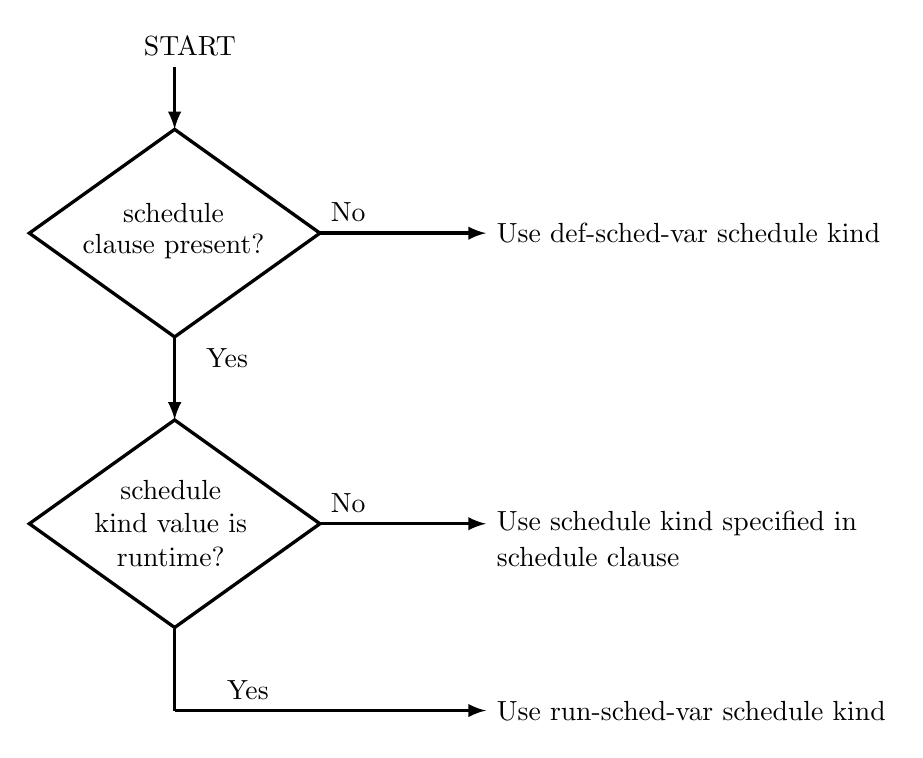
\begin{tikzpicture}
\pgftransformxscale{1.000000}
\pgftransformyscale{-1.000000}
\definecolor{dialinecolor}{rgb}{0.000000, 0.000000, 0.000000}
\pgfsetstrokecolor{dialinecolor}
\definecolor{dialinecolor}{rgb}{1.000000, 1.000000, 1.000000}
\pgfsetfillcolor{dialinecolor}
\definecolor{dialinecolor}{rgb}{1.000000, 1.000000, 1.000000}
\pgfsetfillcolor{dialinecolor}
\fill (18.500000\du,7.000000\du)--(22.000000\du,9.500000\du)--(18.500000\du,12.000000\du)--(15.000000\du,9.500000\du)--cycle;
\pgfsetlinewidth{0.080000\du}
\pgfsetdash{}{0pt}
\pgfsetdash{}{0pt}
\pgfsetmiterjoin
\definecolor{dialinecolor}{rgb}{0.000000, 0.000000, 0.000000}
\pgfsetstrokecolor{dialinecolor}
\draw (18.500000\du,7.000000\du)--(22.000000\du,9.500000\du)--(18.500000\du,12.000000\du)--(15.000000\du,9.500000\du)--cycle;
% setfont left to latex
\definecolor{dialinecolor}{rgb}{0.000000, 0.000000, 0.000000}
\pgfsetstrokecolor{dialinecolor}
\node at (18.500000\du,9.695000\du){};
\pgfsetlinewidth{0.080000\du}
\pgfsetdash{}{0pt}
\pgfsetdash{}{0pt}
\pgfsetbuttcap
{
\definecolor{dialinecolor}{rgb}{0.000000, 0.000000, 0.000000}
\pgfsetfillcolor{dialinecolor}
% was here!!!
\pgfsetarrowsend{latex}
\definecolor{dialinecolor}{rgb}{0.000000, 0.000000, 0.000000}
\pgfsetstrokecolor{dialinecolor}
\draw (18.500000\du,12.000000\du)--(18.500000\du,14.000000\du);
}
\pgfsetlinewidth{0.080000\du}
\pgfsetdash{}{0pt}
\pgfsetdash{}{0pt}
\pgfsetbuttcap
{
\definecolor{dialinecolor}{rgb}{0.000000, 0.000000, 0.000000}
\pgfsetfillcolor{dialinecolor}
% was here!!!
\pgfsetarrowsend{latex}
\definecolor{dialinecolor}{rgb}{0.000000, 0.000000, 0.000000}
\pgfsetstrokecolor{dialinecolor}
\draw (22.000000\du,16.500000\du)--(26.000000\du,16.500000\du);
}
% setfont left to latex
\definecolor{dialinecolor}{rgb}{0.000000, 0.000000, 0.000000}
\pgfsetstrokecolor{dialinecolor}
\node[anchor=west] at (20.000000\du,10.000000\du){};
\pgfsetlinewidth{0.080000\du}
\pgfsetdash{}{0pt}
\pgfsetdash{}{0pt}
\pgfsetbuttcap
{
\definecolor{dialinecolor}{rgb}{0.000000, 0.000000, 0.000000}
\pgfsetfillcolor{dialinecolor}
% was here!!!
\pgfsetarrowsend{latex}
\definecolor{dialinecolor}{rgb}{0.000000, 0.000000, 0.000000}
\pgfsetstrokecolor{dialinecolor}
\draw (18.500000\du,5.500000\du)--(18.500000\du,7.000000\du);
}
% setfont left to latex
\definecolor{dialinecolor}{rgb}{0.000000, 0.000000, 0.000000}
\pgfsetstrokecolor{dialinecolor}
\node[anchor=west] at (31.000000\du,12.000000\du){};
\definecolor{dialinecolor}{rgb}{1.000000, 1.000000, 1.000000}
\pgfsetfillcolor{dialinecolor}
\fill (18.500000\du,14.000000\du)--(22.000000\du,16.500000\du)--(18.500000\du,19.000000\du)--(15.000000\du,16.500000\du)--cycle;
\pgfsetlinewidth{0.080000\du}
\pgfsetdash{}{0pt}
\pgfsetdash{}{0pt}
\pgfsetmiterjoin
\definecolor{dialinecolor}{rgb}{0.000000, 0.000000, 0.000000}
\pgfsetstrokecolor{dialinecolor}
\draw (18.500000\du,14.000000\du)--(22.000000\du,16.500000\du)--(18.500000\du,19.000000\du)--(15.000000\du,16.500000\du)--cycle;
% setfont left to latex
\definecolor{dialinecolor}{rgb}{0.000000, 0.000000, 0.000000}
\pgfsetstrokecolor{dialinecolor}
\node at (18.500000\du,16.695000\du){};
\pgfsetlinewidth{0.080000\du}
\pgfsetdash{}{0pt}
\pgfsetdash{}{0pt}
\pgfsetbuttcap
{
\definecolor{dialinecolor}{rgb}{0.000000, 0.000000, 0.000000}
\pgfsetfillcolor{dialinecolor}
% was here!!!
\pgfsetarrowsend{latex}
\definecolor{dialinecolor}{rgb}{0.000000, 0.000000, 0.000000}
\pgfsetstrokecolor{dialinecolor}
\draw (22.000000\du,9.500000\du)--(26.000000\du,9.500000\du);
}
\pgfsetlinewidth{0.080000\du}
\pgfsetdash{}{0pt}
\pgfsetdash{}{0pt}
\pgfsetbuttcap
{
\definecolor{dialinecolor}{rgb}{0.000000, 0.000000, 0.000000}
\pgfsetfillcolor{dialinecolor}
% was here!!!
\definecolor{dialinecolor}{rgb}{0.000000, 0.000000, 0.000000}
\pgfsetstrokecolor{dialinecolor}
\draw (18.500000\du,19.040000\du)--(18.500000\du,21.000000\du);
}
\pgfsetlinewidth{0.080000\du}
\pgfsetdash{}{0pt}
\pgfsetdash{}{0pt}
\pgfsetbuttcap
{
\definecolor{dialinecolor}{rgb}{0.000000, 0.000000, 0.000000}
\pgfsetfillcolor{dialinecolor}
% was here!!!
\pgfsetarrowsend{latex}
\definecolor{dialinecolor}{rgb}{0.000000, 0.000000, 0.000000}
\pgfsetstrokecolor{dialinecolor}
\draw (18.500000\du,21.000000\du)--(26.000000\du,21.000000\du);
}
% setfont left to latex
\definecolor{dialinecolor}{rgb}{0.000000, 0.000000, 0.000000}
\pgfsetstrokecolor{dialinecolor}
\node[anchor=west] at (17.500000\du,5.000000\du){START};
% setfont left to latex
\definecolor{dialinecolor}{rgb}{0.000000, 0.000000, 0.000000}
\pgfsetstrokecolor{dialinecolor}
\node at (18.471967\du,9.021967\du){\code{schedule} 
};
% setfont left to latex
\definecolor{dialinecolor}{rgb}{0.000000, 0.000000, 0.000000}
\pgfsetstrokecolor{dialinecolor}
\node at (18.471967\du,9.821967\du){clause present?};
% setfont left to latex
\definecolor{dialinecolor}{rgb}{0.000000, 0.000000, 0.000000}
\pgfsetstrokecolor{dialinecolor}
\node at (18.408579\du,15.687353\du){schedule};
% setfont left to latex
\definecolor{dialinecolor}{rgb}{0.000000, 0.000000, 0.000000}
\pgfsetstrokecolor{dialinecolor}
\node at (18.408579\du,16.487353\du){kind value is};
% setfont left to latex
\definecolor{dialinecolor}{rgb}{0.000000, 0.000000, 0.000000}
\pgfsetstrokecolor{dialinecolor}
\node at (18.408579\du,17.287353\du){\code{runtime}?};
% setfont left to latex
\definecolor{dialinecolor}{rgb}{0.000000, 0.000000, 0.000000}
\pgfsetstrokecolor{dialinecolor}
\node[anchor=west] at (26.000000\du,9.500000\du){Use \plc{def-sched-var} schedule kind};
% setfont left to latex
\definecolor{dialinecolor}{rgb}{0.000000, 0.000000, 0.000000}
\pgfsetstrokecolor{dialinecolor}
\node[anchor=west] at (26.000000\du,16.500000\du){Use schedule kind specified in 
};
% setfont left to latex
\definecolor{dialinecolor}{rgb}{0.000000, 0.000000, 0.000000}
\pgfsetstrokecolor{dialinecolor}
\node[anchor=west] at (26.000000\du,17.300000\du){\code{schedule} clause};
% setfont left to latex
\definecolor{dialinecolor}{rgb}{0.000000, 0.000000, 0.000000}
\pgfsetstrokecolor{dialinecolor}
\node[anchor=west] at (26.000000\du,21.000000\du){Use \plc{run-sched-var} schedule kind};
% setfont left to latex
\definecolor{dialinecolor}{rgb}{0.000000, 0.000000, 0.000000}
\pgfsetstrokecolor{dialinecolor}
\node[anchor=west] at (22.000000\du,9.000000\du){No};
% setfont left to latex
\definecolor{dialinecolor}{rgb}{0.000000, 0.000000, 0.000000}
\pgfsetstrokecolor{dialinecolor}
\node[anchor=west] at (19.000000\du,12.500000\du){Yes};
% setfont left to latex
\definecolor{dialinecolor}{rgb}{0.000000, 0.000000, 0.000000}
\pgfsetstrokecolor{dialinecolor}
\node[anchor=west] at (22.000000\du,16.000000\du){No};
% setfont left to latex
\definecolor{dialinecolor}{rgb}{0.000000, 0.000000, 0.000000}
\pgfsetstrokecolor{dialinecolor}
\node[anchor=west] at (19.500000\du,20.500000\du){Yes};
\end{tikzpicture}

\end{quote}
\caption{Determining the \code{schedule} for a Worksharing Loop\label{fig:schedule loop}}
\end{figure}











\subsection{\code{sections} Construct}
\label{subsec:sections Construct}
\index{sections@{\code{sections}}}
\index{constructs!sections@{\code{sections}}}
\summary
The \code{sections} construct is a non-iterative worksharing construct that contains a set of 
structured blocks that are to be distributed among and executed by the threads in a team. 
Each structured block is executed once by one of the threads in the team in the context 
of its implicit task.

\syntax
\begin{ccppspecific}
The syntax of the \code{sections} construct is as follows:

\begin{boxedcode}
\#pragma omp sections \plc{[clause[ [},\plc{] clause] ... ] new-line}
   \{
   \plc{[}\#pragma omp section \plc{new-line}\plc{]}
      \plc{structured-block}
   \plc{[}\#pragma omp section \plc{new-line}
      \plc{structured-block]}
   \plc{...}
   \}
\end{boxedcode}

where \plc{clause} is one of the following: 

\begin{indentedcodelist}
private(\plc{list})
firstprivate(\plc{list})
lastprivate(\plc{[ lastprivate-modifier}:\plc{] list})
reduction(\plc{reduction-identifier }:\plc{ list})
nowait
\end{indentedcodelist}
\end{ccppspecific}

\needspace{16\baselineskip}
\begin{fortranspecific}
The syntax of the \code{sections} construct is as follows:

\begin{boxedcode}
!\$omp sections \plc{[clause[ [},\plc{] clause] ... ]}
   \plc{[}!\$omp section\plc{]}
      \plc{structured-block}
   \plc{[}!\$omp section
      \plc{structured-block]}
   \plc{...}
!\$omp end sections \plc{[}nowait\plc{]}
\end{boxedcode}

\begin{samepage}
where \plc{clause} is one of the following:

\begin{indentedcodelist}
private(\plc{list})
firstprivate(\plc{list})
lastprivate(\plc{[ lastprivate-modifier}:\plc{] list})
reduction(\plc{reduction-identifier }:\plc{ list})
\end{indentedcodelist}
\end{samepage}
\end{fortranspecific}

\binding
The binding thread set for a \code{sections} region is the current team. A \code{sections} 
region binds to the innermost enclosing \code{parallel} region. Only the threads of the team 
executing the binding \code{parallel} region participate in the execution of the structured 
blocks and the implied barrier of the \code{sections} region if the barrier is not eliminated 
by a \code{nowait} clause.

\descr
Each structured block in the \code{sections} construct is preceded by a \code{section} directive 
except possibly the first block, for which a preceding \code{section} directive is optional.

The method of scheduling the structured blocks among the threads in the team is 
implementation defined.

There is an implicit barrier at the end of a \code{sections} construct unless a \code{nowait} 
clause is specified.

%\tools
\omptWorksharing{sections}{ompt\_work\_sections}

\restrictions
Restrictions to the \code{sections} construct are as follows:

\begin{itemize}
\item Orphaned \code{section} directives are prohibited. That is, the \code{section} directives must 
appear within the \code{sections} construct and must not be encountered elsewhere in the 
\code{sections} region.

\item The code enclosed in a \code{sections} construct must be a structured block. 

\item Only a single \code{nowait} clause can appear on a \code{sections} directive.

\begin{cppspecific}
\item A throw executed inside a \code{sections} region must cause execution to resume within 
the same section of the \code{sections} region, and the same thread that threw the 
exception must catch it.
\end{cppspecific}
\end{itemize}

\crossreferences
\begin{itemize}
\item \code{private}, \code{firstprivate}, \code{lastprivate}, and \code{reduction} clauses, see 
\specref{subsec:Data-Sharing Attribute Clauses}.

\item \code{ompt\_scope\_begin} and \code{ompt\_scope\_end}, see
  \specref{sec:ompt_scope_endpoint_t}.

\item \code{ompt\_work\_sections}, see \specref{sec:ompt_work_type_t}.

\item \code{ompt\_callback\_work\_t}, see 
\specref{sec:ompt_callback_work_t}.
\end{itemize}










\subsection{\code{single} Construct}
\index{single@{\code{single}}}
\index{constructs!single@{\code{single}}}
\label{subsec:single Construct}
\summary
The \code{single} construct specifies that the associated structured block is executed by only 
one of the threads in the team (not necessarily the master thread), in the context of its 
implicit task. The other threads in the team, which do not execute the block, wait at an 
implicit barrier at the end of the \code{single} construct unless a \code{nowait} clause is specified.

\syntax
\begin{ccppspecific}
The syntax of the single construct is as follows:

\begin{boxedcode}
\#pragma omp single \plc{[clause[ [},\plc{] clause] ... ] new-line}
   \plc{structured-block}
\end{boxedcode}

\begin{samepage}
where \plc{clause} is one of the following:

\begin{indentedcodelist}
private(\plc{list})
firstprivate(\plc{list})
copyprivate(\plc{list})
nowait
\end{indentedcodelist}
\end{samepage}
\end{ccppspecific}

\begin{fortranspecific}
The syntax of the \code{single} construct is as follows:

\begin{boxedcode}
!\$omp single \plc{[clause[ [},\plc{] clause] ... ]}
   \plc{structured-block} 
!\$omp end single \plc{[end\_clause[ [},\plc{] end\_clause] ... ]}
\end{boxedcode}

where \plc{clause} is one of the following:

\begin{indentedcodelist}
private(\plc{list})
firstprivate(\plc{list})
\end{indentedcodelist}

and \plc{end\_clause} is one of the following: 

\begin{indentedcodelist}
copyprivate(\plc{list})
nowait
\end{indentedcodelist}
\end{fortranspecific}

\binding
The binding thread set for a \code{single} region is the current team. A \code{single} region 
binds to the innermost enclosing \code{parallel} region. Only the threads of the team 
executing the binding \code{parallel} region participate in the execution of the structured 
block and the implied barrier of the \code{single} region if the barrier is not eliminated by a 
\code{nowait} clause.

\descr
Only one of the encountering threads will execute the structured block associated with the \code{single}
construct. The method of choosing a thread to execute the structured block each time the team encounters the construct
is implementation defined. There is an implicit barrier at the end of the \code{single} construct unless a 
\code{nowait} clause is specified. 

\events

The \plc{single-begin} event occurs after an \code{implicit task} encounters a 
\code{single} construct but before the task starts the execution of the structured 
block of the \code{single} region.

The \plc{single-end} event occurs after a \code{single} region finishes execution of the structured block 
but before resuming execution of the encountering implicit task.


\tools

A thread dispatches a registered \code{ompt\_callback\_work}
callback for each occurrence of \plc{single-begin} and
\plc{single-end} events in that thread. The callback has type signature
\code{ompt\_callback\_work\_t}. The callback receives
\code{ompt\_scope\_begin} or \code{ompt\_scope\_end} 
as its \plc{endpoint} argument, as appropriate, and
\code{ompt\_work\_single\_executor} or \code{ompt\_work\_single\_other} 
as its \plc{wstype} argument.

\restrictions
Restrictions to the \code{single} construct are as follows: 

\begin{itemize}
\item The \code{copyprivate} clause must not be used with the \code{nowait} clause.

\item At most one \code{nowait} clause can appear on a \code{single} construct.

\begin{cppspecific}
\item A throw executed inside a \code{single} region must cause execution to resume within the 
same \code{single} region, and the same thread that threw the exception must catch it.
\end{cppspecific}
\end{itemize}


\crossreferences
\begin{itemize}
\item \code{private} and \code{firstprivate} clauses, see 
\specref{subsec:Data-Sharing Attribute Clauses}.

\item \code{copyprivate} clause, see 
\specref{subsubsec:copyprivate clause}.

\item \code{ompt\_scope\_begin} and \code{ompt\_scope\_end}, see
  \specref{sec:ompt_scope_endpoint_t}.

\item \code{ompt\_work\_single\_executor} and \code{ompt\_work\_single\_other}, see
\specref{sec:ompt_work_type_t}.

\item \code{ompt\_callback\_work\_t},
\specref{sec:ompt_callback_work_t}.

\end{itemize}













% Here we need to force the blue marker lower, and force the subsection header higher
% in order to reduce the space between the marker and the header, per Richard:
\begin{samepage}
\vspace{3\baselineskip}
\fortranspecificstart
\vspace{-3\baselineskip}
\subsection{\code{workshare} Construct}
\index{workshare@{\code{workshare}}}
\index{constructs!workshare@{\code{workshare}}}
\label{subsec:workshare Construct}
\summary
The \code{workshare} construct divides the execution of the enclosed structured block into 
separate units of work, and causes the threads of the team to share the work such that 
each unit is executed only once by one thread, in the context of its implicit task.
\end{samepage}

\begin{samepage}
\syntax
The syntax of the \code{workshare} construct is as follows:

\begin{boxedcode}
!\$omp workshare
    \plc{structured-block} 
!\$omp end workshare \plc{[}nowait\plc{]}
\end{boxedcode}
\end{samepage}

The enclosed structured block must consist of only the following:

\begin{itemize}
\item array assignments 

\item scalar assignments 

\item \code{FORALL} statements

\item \code{FORALL} constructs 

\item \code{WHERE} statements

\item \code{WHERE} constructs

\item \code{atomic} constructs

\item \code{critical} constructs

\item \code{parallel} constructs
\end{itemize}

Statements contained in any enclosed \code{critical} construct are also subject to these 
restrictions. Statements in any enclosed \code{parallel} construct are not restricted.

\binding
The binding thread set for a \code{workshare} region is the current team. A \code{workshare} 
region binds to the innermost enclosing \code{parallel} region. Only the threads of the team 
executing the binding \code{parallel} region participate in the execution of the units of 
work and the implied barrier of the \code{workshare} region if the barrier is not eliminated 
by a \code{nowait} clause.
% blue line floater at top of this page for "Fortran, cont."
\begin{figure}[t!]
\linewitharrows{-1}{dashed}{Fortran (cont.)}{8em}
\end{figure}

\descr
There is an implicit barrier at the end of a \code{workshare} construct unless a \code{nowait} 
clause is specified.

An implementation of the \code{workshare} construct must insert any synchronization that is 
required to maintain standard Fortran semantics. For example, the effects of one 
statement within the structured block must appear to occur before the execution of 
succeeding statements, and the evaluation of the right hand side of an assignment must 
appear to complete prior to the effects of assigning to the left hand side.

The statements in the \code{workshare} construct are divided into units of work as follows:

\begin{itemize}
\item For array expressions within each statement, including transformational array 
intrinsic functions that compute scalar values from arrays:

\begin{itemize} % nested level
\item Evaluation of each element of the array expression, including any references to 
\code{ELEMENTAL} functions, is a unit of work.

\item Evaluation of transformational array intrinsic functions may be freely subdivided 
into any number of units of work.
\end{itemize}

\item For an array assignment statement, the assignment of each element is a unit of work.

\item For a scalar assignment statement, the assignment operation is a unit of work.

\item For a \code{WHERE} statement or construct, the evaluation of the mask expression and the 
masked assignments are each a unit of work.

\item For a \code{FORALL} statement or construct, the evaluation of the mask expression, 
expressions occurring in the specification of the iteration space, and the masked 
assignments are each a unit of work

\item For an \code{atomic} construct, the atomic operation on the storage location designated as 
\plc{x} is a unit of work.

\item For a \code{critical} construct, the construct is a single unit of work.

\item For a \code{parallel} construct, the construct is a unit of work with respect to the 
\code{workshare} construct. The statements contained in the \code{parallel} construct are 
executed by a new thread team.

\item If none of the rules above apply to a portion of a statement in the structured block, 
then that portion is a unit of work.
\end{itemize}

The transformational array intrinsic functions are \code{MATMUL}, \code{DOT\_PRODUCT}, \code{SUM}, 
\code{PRODUCT}, \code{MAXVAL}, \code{MINVAL}, \code{COUNT}, 
\code{ANY}, \code{ALL}, \code{SPREAD}, \code{PACK}, \code{UNPACK}, 
\code{RESHAPE}, \code{TRANSPOSE}, \code{EOSHIFT}, \code{CSHIFT}, \code{MINLOC}, and \code{MAXLOC}.

It is unspecified how the units of work are assigned to the threads executing a 
\code{workshare} region.

If an array expression in the block references the value, association status, or allocation 
status of private variables, the value of the expression is undefined, unless the same 
value would be computed by every thread.

If an array assignment, a scalar assignment, a masked array assignment, or a \code{FORALL} 
assignment assigns to a private variable in the block, the result is unspecified.

The \code{workshare} directive causes the sharing of work to occur only in the \code{workshare} 
construct, and not in the remainder of the \code{workshare} region.

%\tools
\omptWorksharing{workshare}{ompt\_work\_workshare}

\begin{samepage}
\restrictions
The following restrictions apply to the \code{workshare} construct:

\begin{itemize}
\item All array assignments, scalar assignments, and masked array assignments must be 
intrinsic assignments.

\item The construct must not contain any user defined function calls unless the function is 
\code{ELEMENTAL}.
\end{itemize}
\fortranspecificend
\end{samepage}

\crossreferences
\begin{itemize}
\item \code{ompt\_scope\_begin} and \code{ompt\_scope\_end}, see
  \specref{sec:ompt_scope_endpoint_t}.
\item \code{ompt\_work\_workshare}, see \specref{sec:ompt_work_type_t}.
\item \code{ompt\_callback\_work\_t}, see
\specref{sec:ompt_callback_work_t}.
\end{itemize}

\filbreak
